\documentclass{article}

% Add custom.sty from the main directory
\usepackage{../../custom}

\title{Homework 3 - Segmentation and Homography}
\author{Naomi Derel, 325324994 
\and Sagi Ben Lulu, 207031493}
\date{08.01.2025}

\begin{document}

\maketitle

\section*{Question 1 - Image Segmentation}

\subsection*{1.1 - Load Images}

\begin{figure}[h!]
    \centering
    \begin{minipage}{0.45\textwidth}
        \centering
        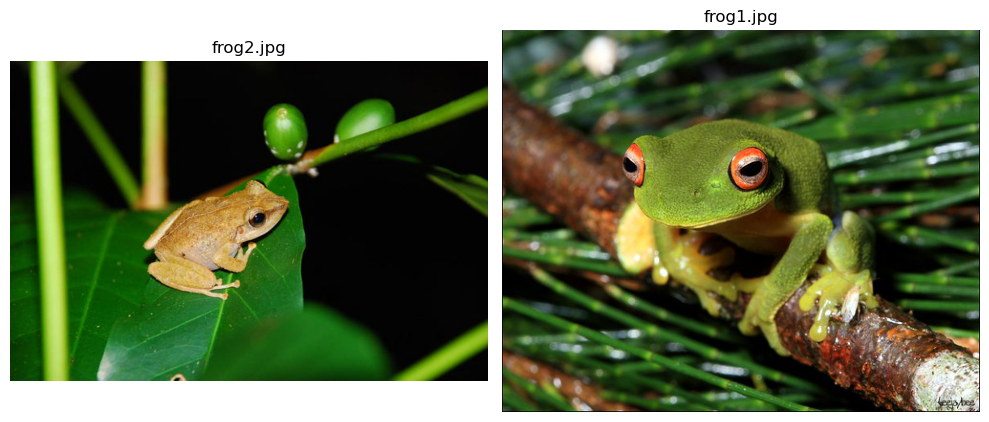
\includegraphics[width=\textwidth]{../output/1.1_frog.png}
        \caption{Images of Frogs}
        \label{fig:1_1_frog}
    \end{minipage}
    \hfill
    \begin{minipage}{0.5\textwidth}
        \centering
        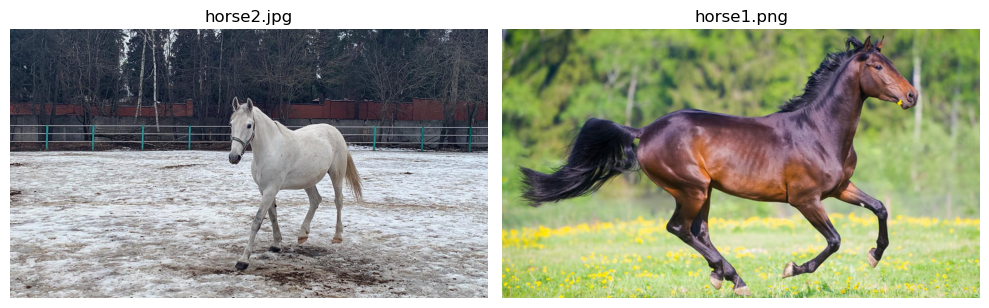
\includegraphics[width=\textwidth]{../output/1.1_horse.png}
        \caption{Images of Horses}
        \label{fig:1_1_horse}
    \end{minipage}
\end{figure}

\subsection*{1.2 - Classical \& Deep Learning Segmentation}

The classic method for segmentation we choose is watershed algorithm, and the deep learning-based method we choose is a pretrained model from torchvision deeplabv3-resnet101.

\subsubsection*{Classical Method - Watershed Algorithm}

\begin{figure}[h!]
    \centering
    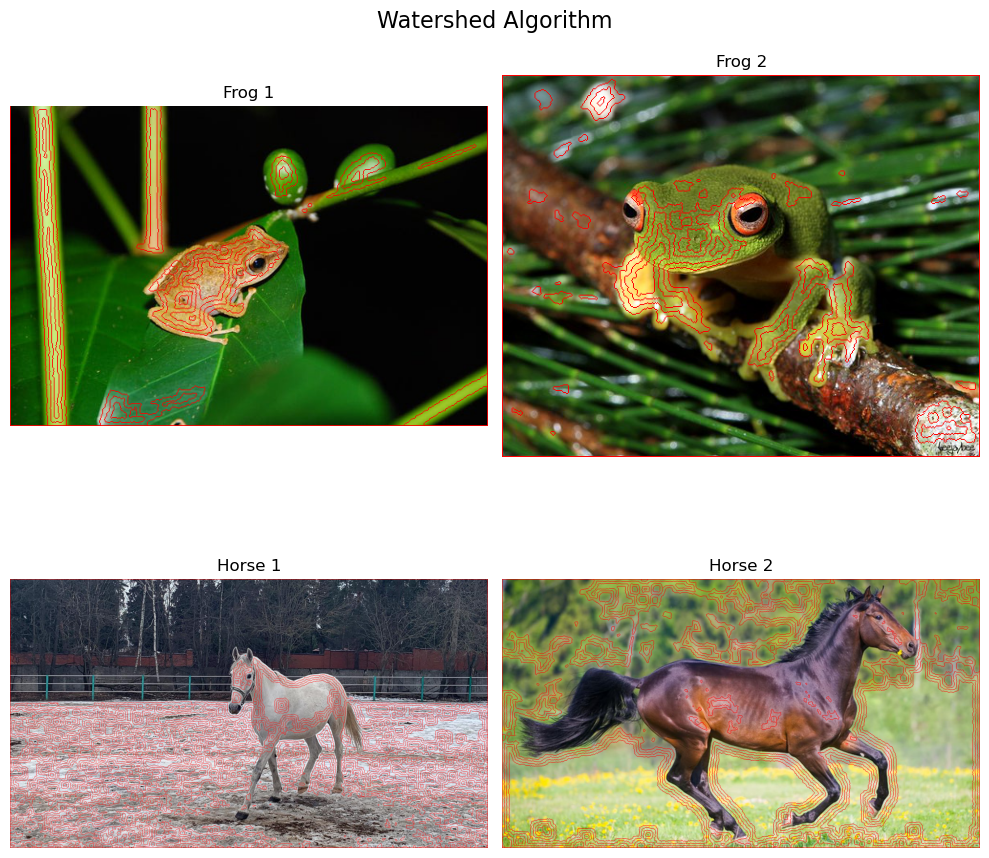
\includegraphics[width=0.5\textwidth]{../output/1.2_watershed.png}
    \caption{Segmentation Results Using the Watershed Algorithm}
    \label{fig:1_2_watershed}
\end{figure}

The watershed algorithm finds local minimas in the gradient image and then iteratively add neighboring pixels to the same area (segmentation) until reaches a pixel that belongs to a different area and this is the boundary between areas. 

The results of the segmentation are in Figure~\ref{fig:1_2_watershed}.

\subsubsection*{Deep Learning Method - ResNet}

deeplabv3-resnet101 uses a resnet101 network as a backbone for the segmentation to find lower dimension features, resnet101 is a deep convolutional network that uses skip connections. Then uses Atrous Spatial Pyramid Pooling to upsample the output for segmentation. 

The results of the segmentation are in the following 4 Figures \ref{fig:1_2_resnet1}, \ref{fig:1_2_resnet2}, \ref{fig:1_2_resnet3}, \ref{fig:1_2_resnet4}.

\begin{figure}[h!]
    \centering
    \begin{minipage}{0.45\textwidth}
        \centering
        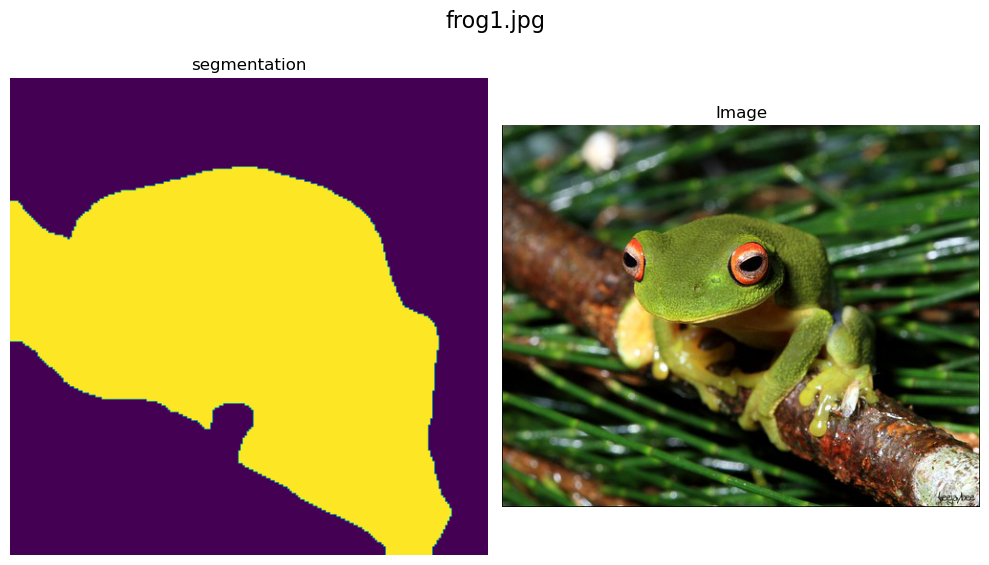
\includegraphics[width=\textwidth]{../output/1.2_rn1.png}
        \caption{Segmentation of Frog 1}
        \label{fig:1_2_resnet1}
    \end{minipage}
    \hfill
    \begin{minipage}{0.45\textwidth}
        \centering
        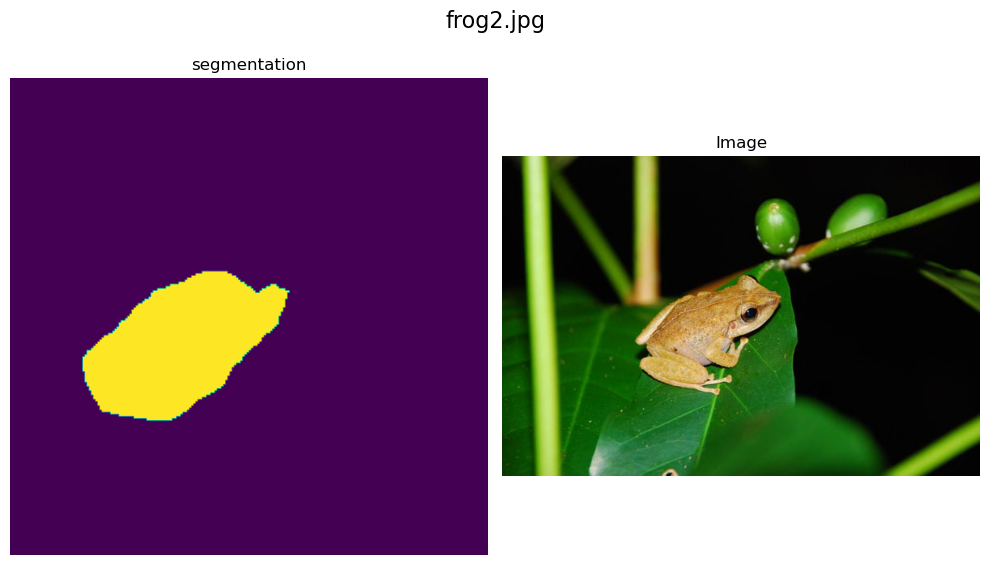
\includegraphics[width=\textwidth]{../output/1.2_rn2.png}
        \caption{Segmentation of Frog 2}
        \label{fig:1_2_resnet2}
    \end{minipage}
\end{figure}

\begin{figure}[h!]
    \centering
    \begin{minipage}{0.45\textwidth}
        \centering
        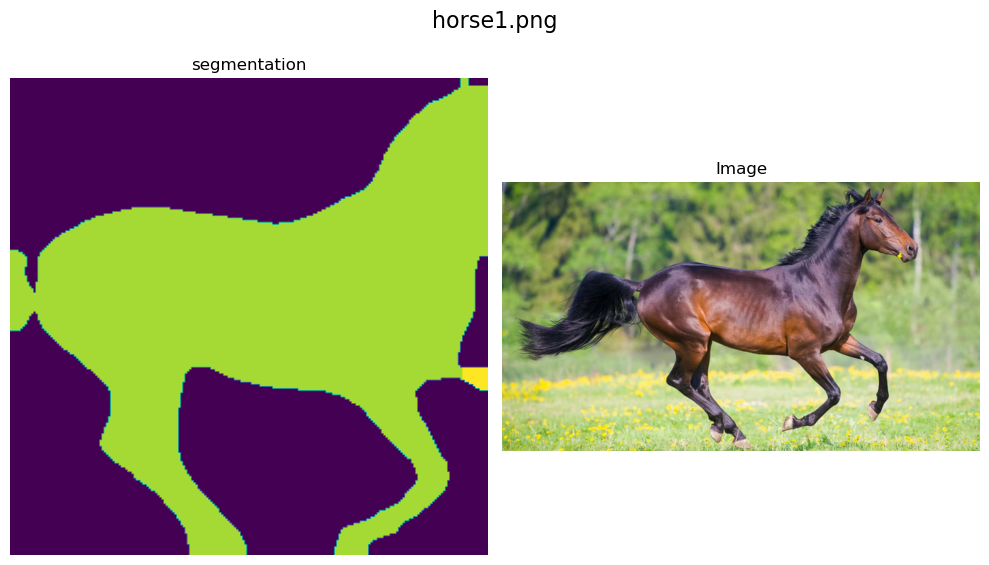
\includegraphics[width=\textwidth]{../output/1.2_rn3.png}
        \caption{Segmentation of Horse 1}
        \label{fig:1_2_resnet3}
    \end{minipage}
    \hfill
    \begin{minipage}{0.45\textwidth}
        \centering
        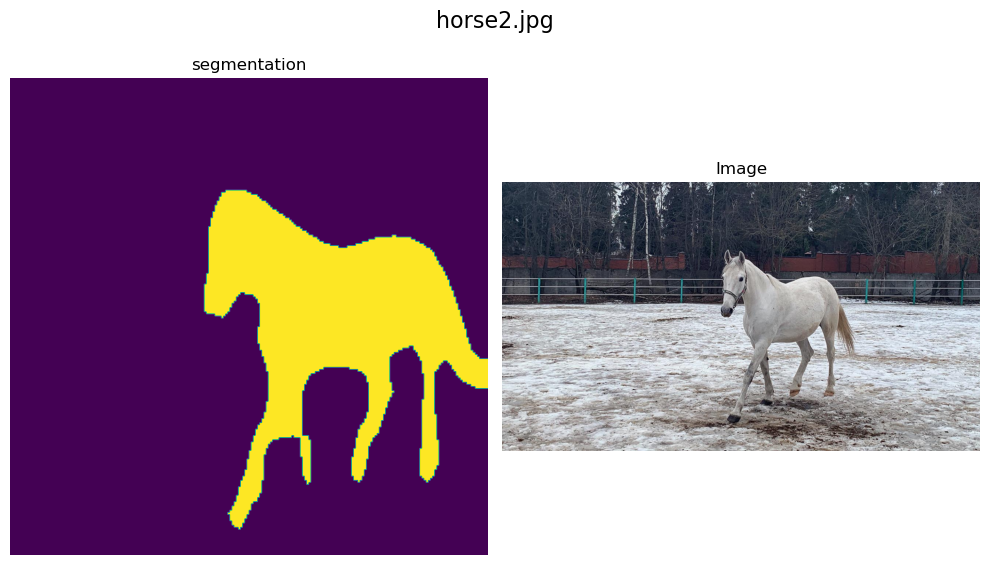
\includegraphics[width=\textwidth]{../output/1.2_rn4.png}
        \caption{Segmentation of Horse 2}
        \label{fig:1_2_resnet4}
    \end{minipage}
\end{figure}

\subsubsection*{Advantages and Disadvantages}

From the results, we can see that the deep learning method is far more accurate than the classical method and provides bounding boxes. However, for the orange frog, the deep learning method does not capture exact details that the classical method does. Additionally, the deep learning method is more computationally expensive and requires a pretrained model, while the classical method is fast and is possible to implement from scratch with limited resources.

\subsection*{1.3 - Additional Images}

We select an image of a human being (\texttt{'lena.jpg'}), an image of a common object - a car, and an image of an uncommon object - a missile. The images are shown in Figures \ref{fig:1_3_imgs}.

\begin{figure}
    \centering
    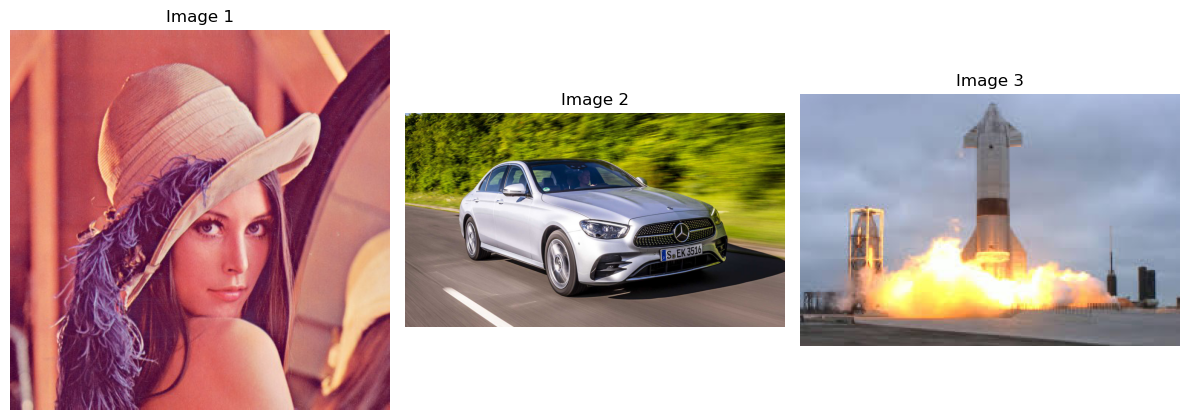
\includegraphics[width=\textwidth]{../output/1.3_imgs.png}
    \caption{Additional Images}
    \label{fig:1_3_imgs}
\end{figure}

\subsection*{1.4 - Segmentation of Additional Images}

The results of both methods of segmentation are shown in Figures \ref{fig:1_4_watershed} and \ref{fig:1_4_resnet}.

\begin{figure}[h!]
    \centering
    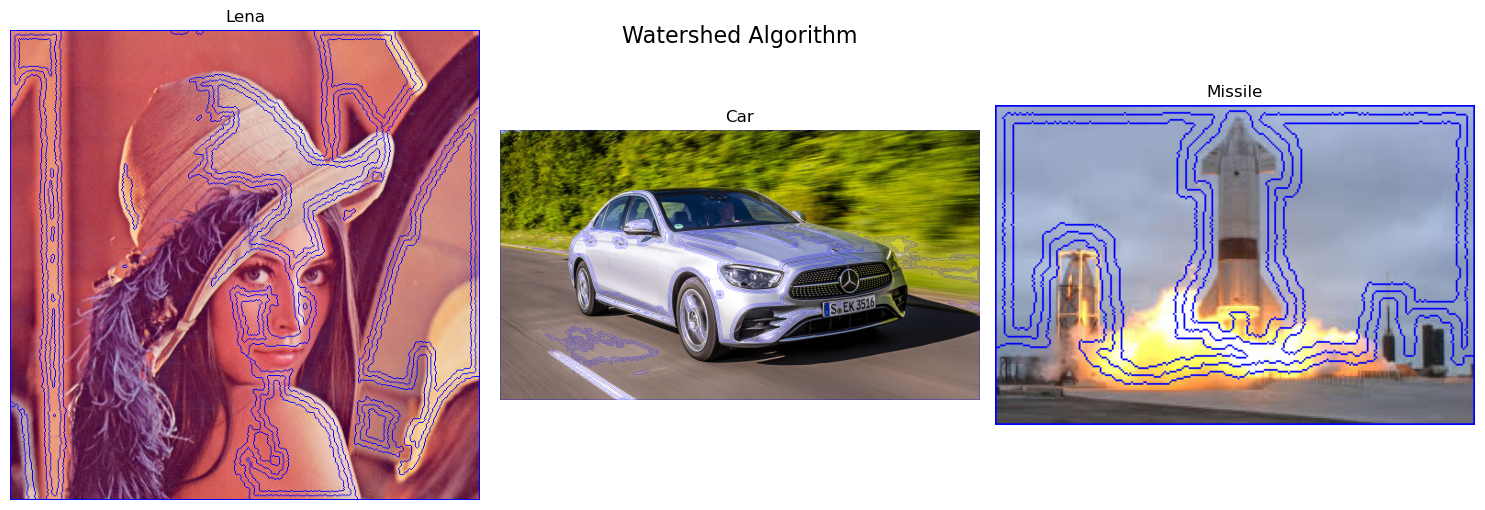
\includegraphics[width=0.5\textwidth]{../output/1.4_watershed.png}
    \caption{Segmentation Results Using the Watershed Algorithm}
    \label{fig:1_4_watershed}
\end{figure}

\begin{figure}[h!]
    \centering
    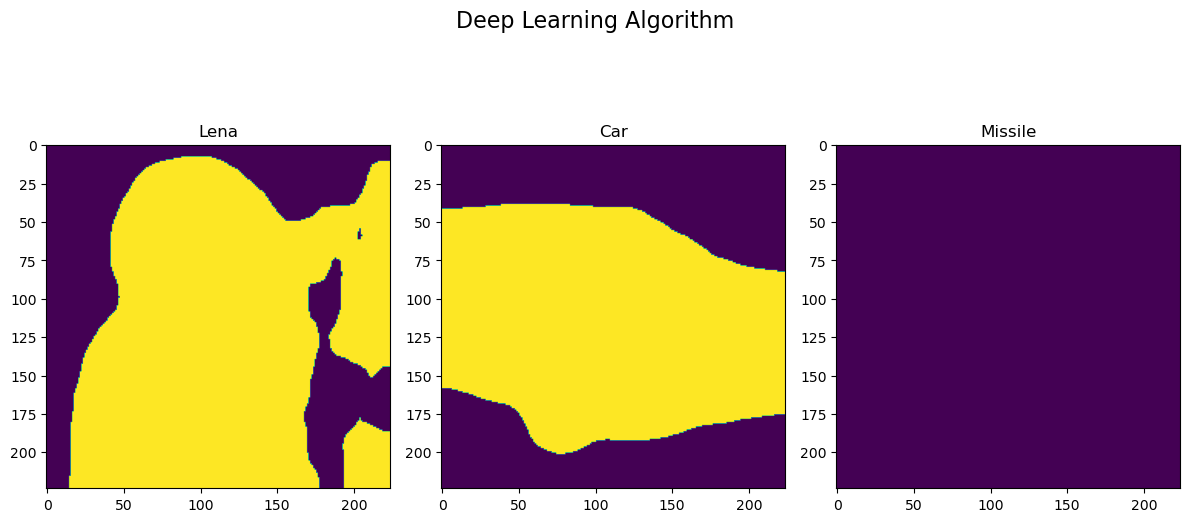
\includegraphics[width=0.5\textwidth]{../output/1.4_deep.png}
    \caption{Segmentation Results Using the ResNet Model}
    \label{fig:1_4_resnet}
\end{figure}

The network method got a lot better results for the person and car but wasn’t able to segment the missile, probably because it is not similar to the training data and therefore the model didn’t learn to classify it.
The Watershed algorithm got similar results for all the images and therefore the performance on the missile image is better than the network method got. We can also see that the algorithm performs better on the homogeneous parts and finds larger areas.

\subsection*{1.5 - Improvment Suggestions}

We can try to apply a smoothing filter before the segmentation, this might help on regions like the horse's tail that are not fully covered but might also get worse results when for example trying to distinguish between objects. Another suggestion is to add an edge image channel, for example to apply a canny edge detector to get another channel, this might help the model learn the boundaries better and get better results around the edges.

\section*{Question 3 - Planar Homographies}

\subsection*{3.0 - SIFT}

\begin{figure}[h!]
    \centering
    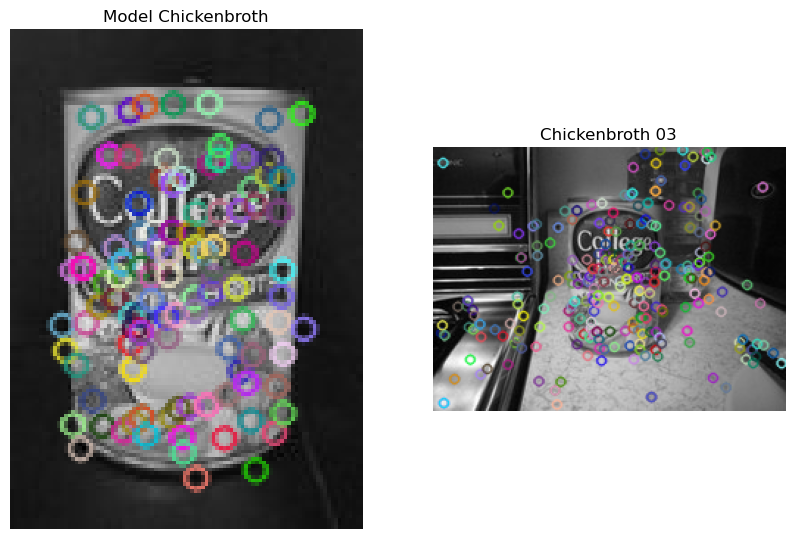
\includegraphics[width=0.5\textwidth]{../output/3.0_sift.png}
    \caption{Descriptor Points on Chickenbroth Model and Counter Images}
    \label{fig:3_1}
\end{figure}

\subsection*{3.1 - Finding Corresponding Points Using SIFT}

\begin{figure}[h!]
    \centering
    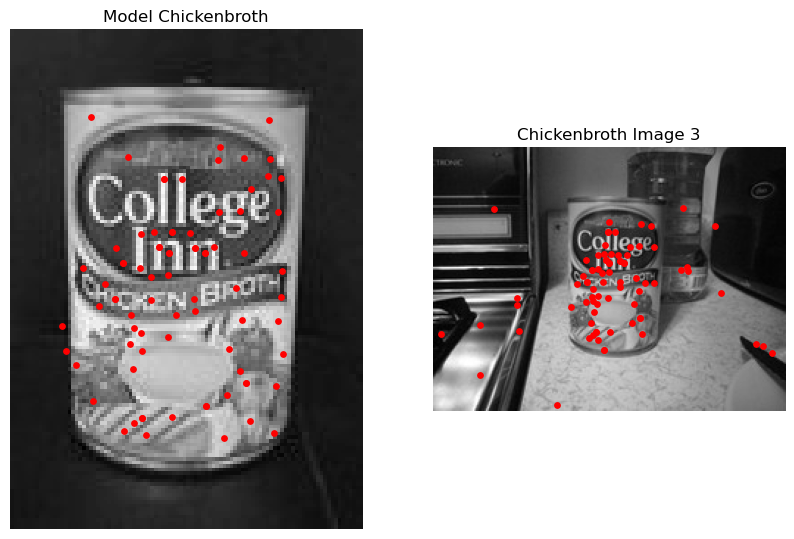
\includegraphics[width=0.5\textwidth]{../output/3.1_cb.png}
    \caption{Corresponding Points on Chickenbroth Model and Counter Images}
    \label{fig:3_1}
\end{figure}

\subsection*{3.2 - Calculating Transformation}

The implemented function to find the homography matrix performs the following steps:
\begin{enumerate}
    \item From given points, constructs the $A$ matrix as seen in lecture. For each point, two rows are defined:
    \[ A = 
    \begin{bmatrix}
        -x & -y & -1 & 0 & 0 & 0 & x'x & x'y & x' \\
        0 & 0 & 0 & -x & -y & -1 & y'x & y'y & y'
    \end{bmatrix}
    \]
    \item Calculate the SVD decomposition of $A$.
    \item Find the minimal singular value and its corresponding column in $V$.
    \item Reshape the column to a $3 \times 3$ matrix $H$ and return it.
\end{enumerate}

The result is projected using the matrix, returned to heterogeneous coordinates and displayed in the image. The result is shown in Figure~\ref{fig:3_2}.

\begin{figure}[h!]
    \centering
    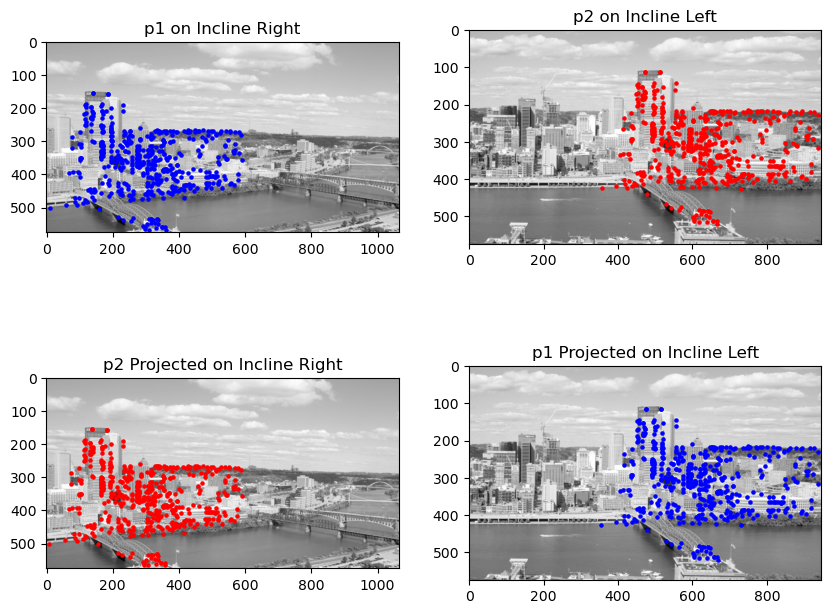
\includegraphics[width=0.8\textwidth]{../output/3.2_incline.png}
    \caption{Homography Transformation of Incline Panorama Images}
    \label{fig:3_2}
\end{figure}

The projection appears to be relatively accurate, with many points matching between the original image (top row) and the relevant projected points (bottom row).

\subsection*{3.3 - Image Warping}

\begin{figure}[h!]
    \centering
    \begin{minipage}{0.45\textwidth}
        \centering
        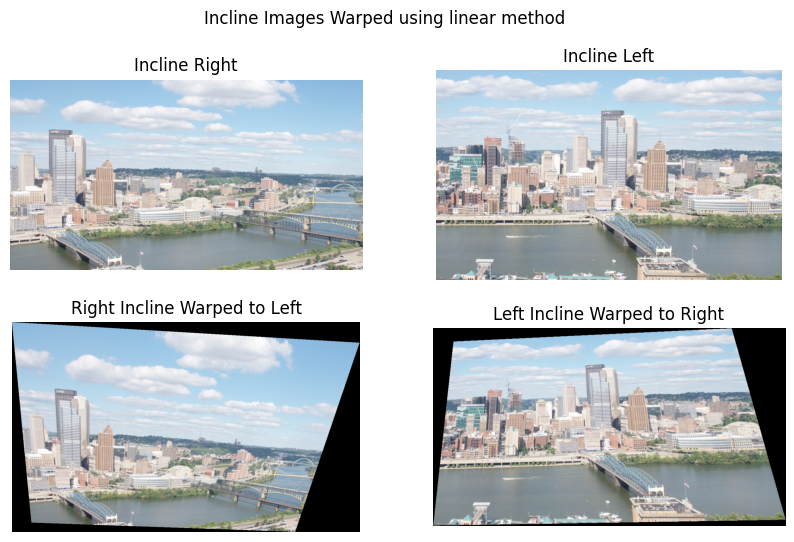
\includegraphics[width=\textwidth]{../output/3.3_linear.png}
        \caption{Linear Interpolation of Incline Panorama Images}
        \label{fig:3_3_linear}
    \end{minipage}
    \hfill
    \begin{minipage}{0.45\textwidth}
        \centering
        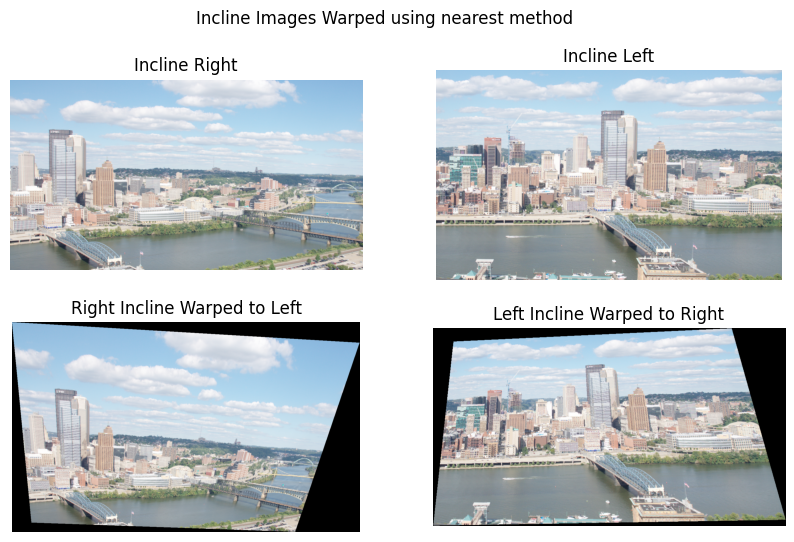
\includegraphics[width=\textwidth]{../output/3.3_nearest.png}
        \caption{Nearest Interpolation of Incline Panorama Images}
        \label{fig:3_3_nearest}
    \end{minipage}
\end{figure}

We first implement a function that computes the necessary dimensions for the output image, which is done by computing the new coordinates of the corners of the image using the homography matrix. This function also updates the homography matrix to shift the image to the origin.

Then, the parameters can be inputted into the warp function, which uses inverted wrapping. The function is implemented using the suggested \texttt{RegularGridInterpolator}, which accepts a method of interpolation. We test the 'linear' method and the 'nearest' method, and the results are shown in Figures \ref{fig:3_3_linear} and \ref{fig:3_3_nearest} respectively.

The results are very similar for both methods. The linear method interpolates between the pixels to create a smoother image, while the nearest method simply takes the nearest pixel value - however in this case, it is hard to notice the difference, likely due to the distance of the incline or quality of the images.


\subsection*{3.4 - Panorama Stitching}

Following the instructions in the question, we assume the input images consist of two images, one of which is wrapped using the \texttt{warpPerspective} function. The images are then overlapped by padding and layering the images on top of each other. The result is shown in Figure~\ref{fig:3_4}.

\begin{figure}[h!]
    \centering
    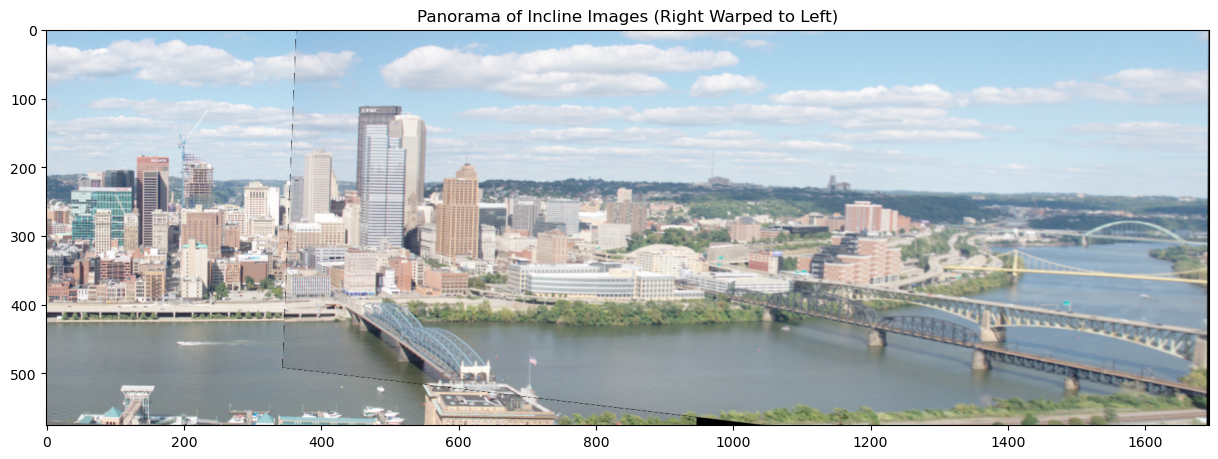
\includegraphics[width=0.8\textwidth]{../output/3.4_panorama.png}
    \caption{Panorama Stitching of Incline Panorama Images}
    \label{fig:3_4}
\end{figure}

\subsection*{3.5 - Several Image Stitching}

First, we show the series of images and the resulting panramas on two domains: the Sintra castle and the beach photos.

We note that for both panoramas, since we are not using any selective point algorithm such as RANSAC, we must carefully utilize only some of the points recieved by the SIFT algorithms, specifically those with the highest confidence. This is because not all matches are correct, and using those to compute the homography matrix results in incomprehensible panoramas with "smeared" images. In practice, we used between 30-100 points to compute the panoramas well.

\subsubsection*{Sintra}

The seperate images of the Sintra castle are shown in Figure~\ref{fig:3_5_sintras}. The resulting panorama is shown in Figure~\ref{fig:3_5_sin_pan}.

\begin{figure}[h!]
    \centering
    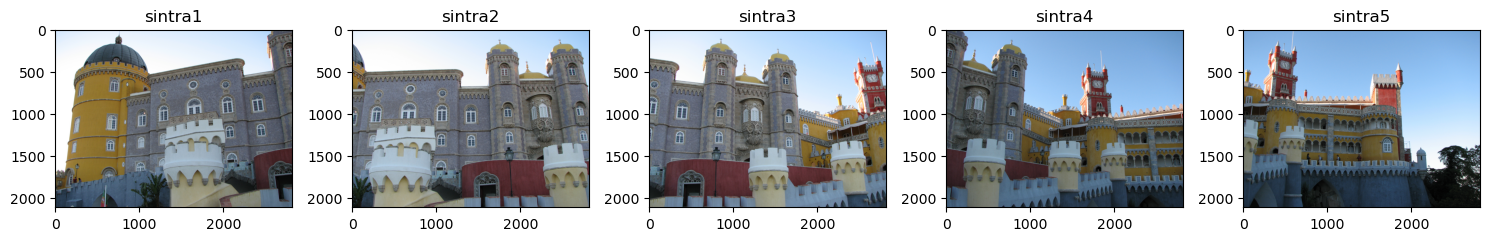
\includegraphics[width=0.8\textwidth]{../output/3.5_sintras.png}
    \caption{5 Images of the Sintra Castle}
    \label{fig:3_5_sintras}
\end{figure}

\begin{figure}[h!]
    \centering
    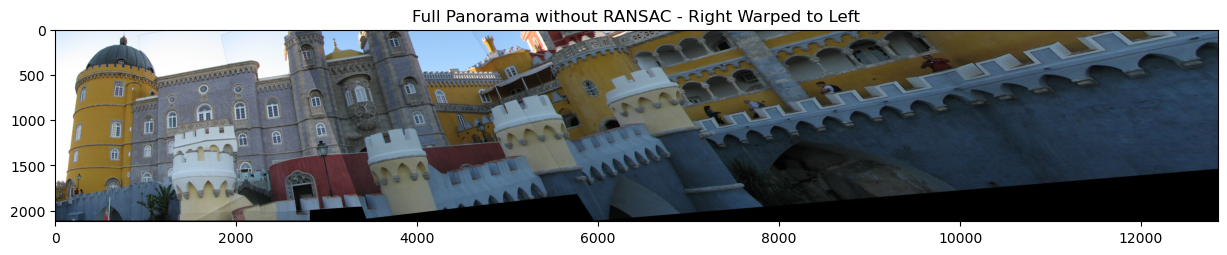
\includegraphics[width=0.8\textwidth]{../output/3.5_sin_pan.png}
    \caption{Panorama of the Sintra Castle}
    \label{fig:3_5_sin_pan}
\end{figure}

\subsubsection*{Beach}

The seperate images of the beach are shown in Figure~\ref{fig:3_5_beaches}. The resulting panorama is shown in Figure~\ref{fig:3_5_beach_pan}.

\begin{figure}[h!]
    \centering
    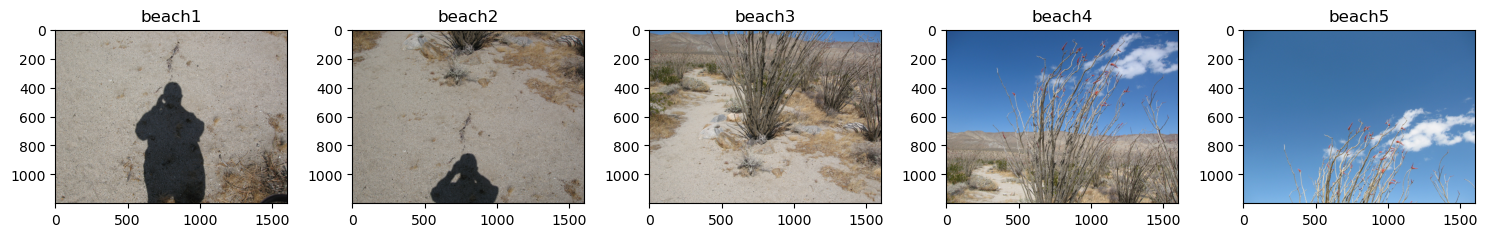
\includegraphics[width=0.8\textwidth]{../output/3.5_beaches.png}
    \caption{5 Images of the Beach}
    \label{fig:3_5_beaches}
\end{figure}

\begin{figure}[h!]
    \centering
    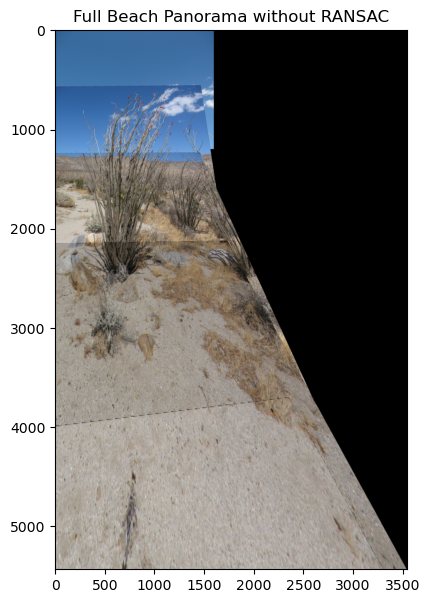
\includegraphics[width=0.4\textwidth]{../output/3.5_beach_pan.png}
    \caption{Panorama of the Beach}
    \label{fig:3_5_beach_pan}
\end{figure}

As the amount of images grow, the panorama becomes more streched out, the points are harder to match, and more information is lost. This is exagerated by each new image attaching to an already warped image which exagerates the angle and makes it harder to match, as the images are not strictly on a single plane and the depth difference interferes.

\subsection*{3.6 - RANSAC}

RANSAC allows for a selection of only the best match points and computation of H according to them. This helps reduce the chances of wrong matches which result in an unclear panorama. Especially, it could be needed when objects in the images are on different planes, when there is noise in the images or when there are similar keypoints in the image and errors are more likely.

\begin{figure}[h!]
    \centering
    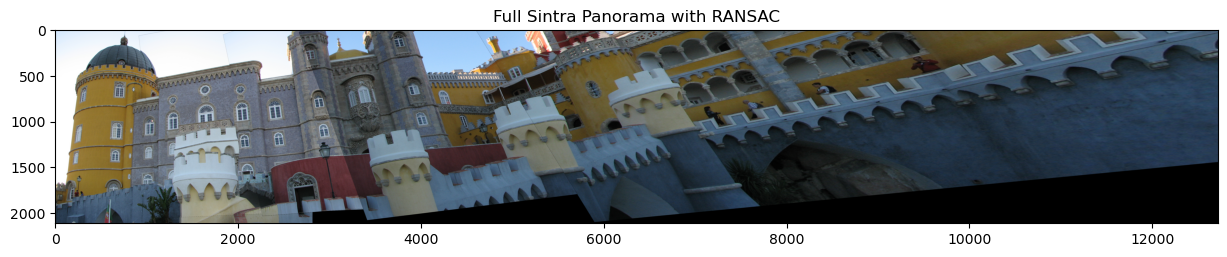
\includegraphics[width=0.8\textwidth]{../output/3.6_sintra.png}
    \caption{Panorama of Sintra with RANSAC}
    \label{fig:3_6_sintra}
\end{figure}

\begin{figure}[h!]
    \centering
    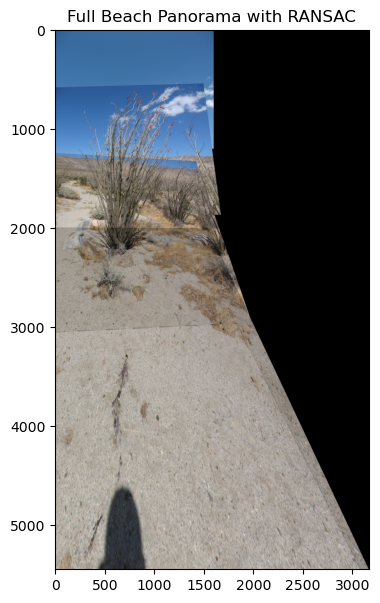
\includegraphics[width=0.4\textwidth]{../output/3.6_beach.png}
    \caption{Panorama of Beach with RANSAC}
    \label{fig:3_6_beach}
\end{figure}

We show the results of the panoramas using the RANSAC algorithm, instead of selecting the first matches with most confidence as done before, in Figures~\ref{fig:3_6_sintra}, \ref{fig:3_6_beach}.


Compared to not using RANSAC, the results on the Sintra images are similar, although there was no need for the careful selection of correct number of matches and so it is less prone to error. On the beach images, the RANSAC algorithm with appropriate parameters allowed for more of the image space to show as the homography matrix became more accurate. This improves the results, and makes them more robust similarly to the Sintra panorama.

These results could be improved further by increasing the iteration number even more and fine tuning the parameters to reach the best results, as trial and error on the beach images shows this can lead to improvement. Further improvement might be achieved through trying different ordering of the panoramic construction to avoid as much loss as possible in the images - this can be seen with the number of matches going down with the number of images stacked on top of each other, and sometimes going out of balance.


\subsection*{3.7 - Creating Our Own Panorama}

We took 3 pictures of the Zisapel building  with only camera rotation differences. Then resized the images to a smaller size (for shorter computation) and created their combined panorama image.

The seperate images of the Zisapel building are shown in Figure~\ref{fig:3_7_zisapels}. The resulting panorama, computed with RANSAC, is shown in Figure~\ref{fig:3_7_pan}.

\begin{figure}[h!]
    \centering
    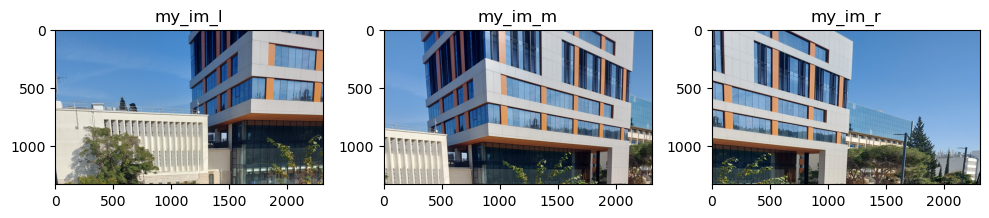
\includegraphics[width=0.8\textwidth]{../output/3.7_buildings.png}
    \caption{3 Images of the Zisapel Building}
    \label{fig:3_7_zisapels}
\end{figure}

\begin{figure}[h!]
    \centering
    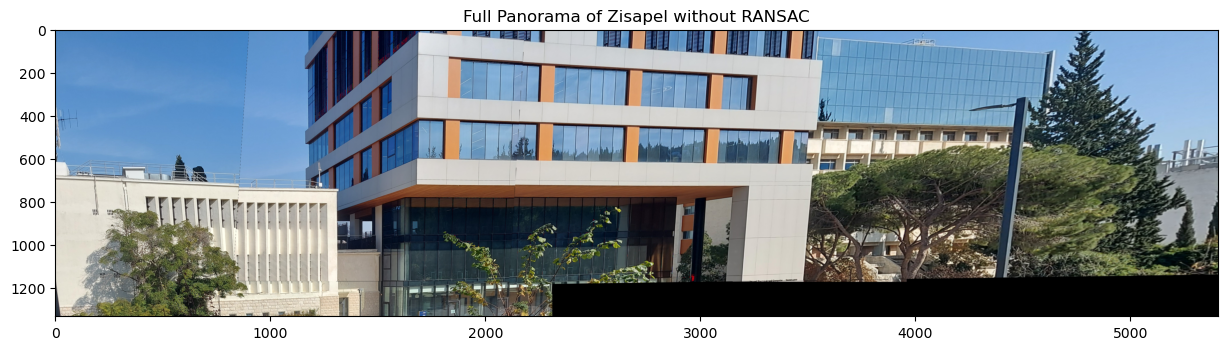
\includegraphics[width=0.8\textwidth]{../output/3.7_pan.png}
    \caption{Panorama of the Zisapel Building}
    \label{fig:3_7_pan}
\end{figure}

This is the best result we achieved, through using the RANSAC algorithm and as many as 2,000 iterations, which allowed for a near perfect alignment of the images, while using the matches without RANSAC didn't work at all and created an incomprehensible image.



\end{document}